\begin{surferPage}[Quártica Kummer]{A Qu\'artica de  Kummer}
Em 1875,  Eduard Kummer colocou explicitamente e pela primeira vez a quest\~ao acerca do n\'umero m\'aximo $\mu(d)$ de singularidades numa superf\'icie de grau $d$,  no seu caso para as superf\'icies de grau $4$, chamadas \emph{qu\'articas}. 
  
 Kummer mostrou que $\mu(4)=16$. Em seguida, Kummer estudou em pormenor as qu\'articas com $16$
    singularidades.
    Uma fam\'ilia  de tais superf\'icies particularmente atraentes \'e dada por:
    \[\bigl(x^2+y^2+z^2-\mu^2\bigr)^2 - \lambda
    \,y_0\,y_1\,y_2\,y_3,\]
    onde $\mu$ \'e um par\^ametro livre e
    $\lambda = \frac{3\mu^2-1}{3-\mu^2}$; os $y_i$ s\~ao os lados de um tetraedro regular {\small
    $y_0=1-z-\sqrt{2}x$, \  
    $y_1=1-z+\sqrt{2}x$, \ 
    $y_2=1+z+\sqrt{2}y$, \ 
    $y_3=1+z-\sqrt{2}y$}
 para tornar a superf\'icie sim\'etrica.
  Nem todos os membros desta fam\'ilia t\^em exatamente $16$ singularidades reais,
  embora a maioria deles tenham:
  \begin{center}
    \vspace*{-0.2cm}\hspace*{-0.2cm}
    \begin{tabular}{@{}c@{\,}c@{\,}c@{\,}c@{\,}c@{}}
      \begin{tabular}{@{}c@{}}
        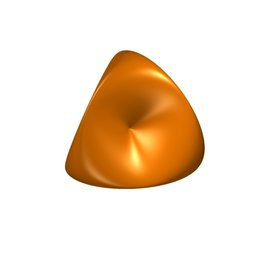
\includegraphics[height=1.4cm]{./../../common/images/kummer_0}
      \end{tabular}
      &
      \begin{tabular}{@{}c@{}}
        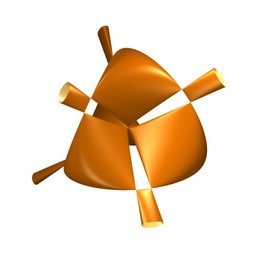
\includegraphics[height=1.4cm]{./../../common/images/kummer_1}
      \end{tabular}
      &
      \begin{tabular}{@{}c@{}}
        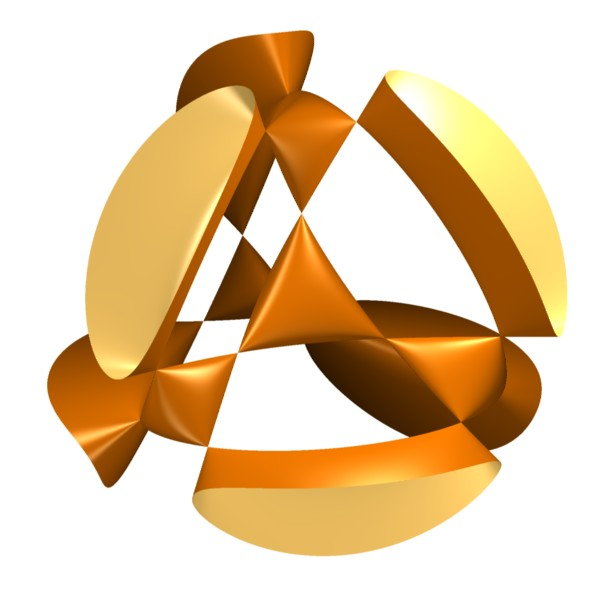
\includegraphics[height=1.4cm]{./../../common/images/kummer_2}
      \end{tabular}
      &
      \begin{tabular}{@{}c@{}}
        
\includegraphics[height=1.4cm]{./../../common/images/kummer_3}
      \end{tabular}
    \end{tabular}
  \end{center}
  \vspace{-0.2cm}  
   Para alguns valores especiais dos par\^ametros, algumas das singularidades podem coincidir.
\end{surferPage}
